\documentclass[11pt,reqno]{amsart}

\usepackage[margin=1.0in]{geometry}
\usepackage[T1]{fontenc}
\usepackage{amsmath,amssymb,amsthm,mathtools}
\usepackage{booktabs,array,multirow}
\usepackage{graphicx}
\usepackage{xcolor}
\usepackage{enumitem}
\usepackage{microtype}
\usepackage{url}
\usepackage[hidelinks,
  pdftitle={Coset-Quotient Compression, Separation-Graph Barriers, and Multi-Kernel Verified Frontiers for Zero-Error Shannon Capacity},
  pdfauthor={Alexander Stephen Donahue},
  pdfsubject={Combinatorics (math.CO); Information Theory (cs.IT); Logic in Computer Science (cs.LO)}
]{hyperref}

\hypersetup{
  colorlinks=true,
  linkcolor=blue!60!black,
  citecolor=teal!70!black,
  urlcolor=blue!65!black
}

\newtheorem{theorem}{Theorem}[section]
\newtheorem{proposition}[theorem]{Proposition}
\newtheorem{lemma}[theorem]{Lemma}
\newtheorem{corollary}[theorem]{Corollary}
\theoremstyle{definition}
\newtheorem{definition}[theorem]{Definition}
\newtheorem{remark}[theorem]{Remark}
\newtheorem{openproblem}[theorem]{Open Problem}

\newcommand{\Z}{\mathbb{Z}}
\newcommand{\N}{\mathbb{N}}
\newcommand{\Q}{\mathbb{Q}}
\newcommand{\R}{\mathbb{R}}
\newcommand{\F}{\mathbb{F}}
\newcommand{\sprod}{\boxtimes}
\newcommand{\Hbpz}{H_{\mathrm{BPZ}}}
\newcommand{\Hstar}{H^*}
\newcommand{\dist}{\mathrm{dist}_n}
\newcommand{\lean}[1]{\nolinkurl{#1}}

\title[Coset-Quotient Compression and Zero-Error Capacity Frontiers]{%
  Coset-Quotient Compression, Separation-Graph Barriers, and Multi-Kernel Verified Frontiers for Zero-Error Shannon Capacity}

\author{Alexander Stephen Donahue}
\address{Independent Researcher, Spokane, WA, USA}
\email{0\_0@0thernes.art}
\urladdr{https://orcid.org/0009-0006-8168-9648}

\date{November 25, 2026}
\subjclass[2020]{Primary 05C69, 94A24; Secondary 05C76, 05C50, 68V20}
\keywords{Shannon capacity, odd cycles, strong graph product, coset-quotient compression, separation calculus, Haemers bound, Schläfli graph, Lean 4 formal verification}

\begin{document}

\begin{abstract}
We establish four interconnected, fully machine-verified advances on the zero-error Shannon capacity of odd cycles and strong graph products.
First, we introduce an algebraic \emph{coset-quotient compression} theory for four-dimensional discrete tori $C_n^{\sprod 4}$: quotienting by two-dimensional subgroups compresses $n^2$-word cosets to single points in two-dimensional quotient tori, proves exact double-counting quotient ceilings, and reveals a sharp structural dichotomy between the classic subgroup $\Hbpz = \langle(1,0,0,2),(0,1,2,0)\rangle$ (forbidden ball size $49$, intra-coset port obstruction) and a newly discovered subgroup $\Hstar = \langle(1,0,0,2),(0,1,0,4)\rangle$ (forbidden ball size $45$, unconditional intra-coset privacy for all odd $n \ge 15$). From this framework we construct two infinite exact-ceiling code families: a helical $\Hbpz$ family for $C_{4m+1}$ ($m \equiv 0,1 \pmod 4$) and an $\Hstar$ staircase family for $C_{8k+1}$ that automatically generates $n^2$-port liftable systems for every odd $k \ge 3$ ($C_{25}, C_{41}, C_{57}, \dots$), alongside a locally-injective Baumert pullback homomorphism $C_{p+2}^{\sprod d} \to C_p^{\sprod d}$ with exact factored cardinality.
Second, combining these algebraic bases with certified port systems and pure-kernel recursive substitution tables, we prove four new world-record lower bounds surpassing the 1971--1973 Baumert--Hales benchmarks:
$\Theta(C_{25}) \ge 12.344196091426841$ ($p=144$),
$\Theta(C_{27}) \ge 13.319390984674515$ ($p=2048$),
$\Theta(C_{29}) \ge 14.319949949077991$ ($p=4$, exact quotient ceiling), and
$\Theta(C_{31}) \ge 15.308776193986504$ ($p=2048$).
Third, we uncover the combinatorial anatomy of the seven-letter separation graph $G_7$ underlying recursive capacity lifts: $G_7$ contains an induced chordless $C_5$, satisfies $\Theta(G_7) = \alpha(G_7) = \bar{\chi}(G_7) = 3$, obeys a sharp weighted fractional-clique-cover barrier ($46875/2$ for $C_{25}$'s 625-port profile), and generalizes to a two-sided heterogeneous composition theorem resolving Open Problem~\#2 of Tandon (\texttt{arXiv:2608.30273}).
Fourth, we develop a zero-Mathlib algebraic theory of upper bounds---the general Haemers rank theorem over any field, an exact integer orthogonal-handle sandwich theorem avoiding floating-point arithmetic, Lovász's $\Theta(C_5)=\sqrt{5}$ via an exact $\Z[\sqrt{5}]$ Gram idempotent, and the first zero-Mathlib, six-kernel verified proof of Haemers's 1979 Schläfli super-multiplicativity paradox ($\Theta(G_{27})\le 3$, $\Theta(\overline{G_{27}})\le 7$, $\Theta(G_{27}\sprod\overline{G_{27}})\ge 27 > 21$).
Every theorem is formalized in standalone Lean~4.35.0 with zero Mathlib dependencies, zero \texttt{sorry}, zero \texttt{native\_decide}, and strict axioms $\subseteq\{\texttt{propext},\texttt{Classical.choice},\texttt{Quot.sound}\}$, replayed across six independent proof kernels and differentially audited in Rust, ISO~C11, and exact-arithmetic Python. Determining exact $\Theta(C_n)$ for odd $n \ge 7$ remains explicitly open.
\end{abstract}

\maketitle

\section{Introduction and Epistemic Architecture}\label{sec:intro}

Introduced by Shannon~\cite{shannon1956zero}, the zero-error capacity of a finite simple graph $G = (V,E)$ is
\[
  \Theta(G) \;:=\; \sup_{d \ge 1} \alpha\bigl(G^{\sprod d}\bigr)^{1/d} \;=\; \lim_{d\to\infty} \alpha\bigl(G^{\sprod d}\bigr)^{1/d},
\]
where $G \sprod H$ denotes the \emph{strong product} (two distinct pairs $(u_1,v_1)\neq(u_2,v_2)$ are adjacent iff both coordinates are equal or adjacent) and $\alpha(\cdot)$ is the independence number. Despite seven decades of progress---including the classical three-dimensional odd-cycle packings of Baumert et al.~\cite{baumert1971combinatorial} and Hales~\cite{hales1973numerical}, Lovász's semidefinite $\vartheta$-function settling $\Theta(C_5)=\sqrt{5}$~\cite{lovasz1979shannon}, Haemers's matrix-rank bound refuting multiplicativity via the Schläfli graph~\cite{haemers1979some}, Schrijver's strengthening~\cite{schrijver1979comparison}, Alon's union non-additivity~\cite{alon1998shannon}, Bohman's limit theorems~\cite{bohman2003limit,bohman2005limit2,bohman2003nontrivial}, Alon--Lubetzky's power-sequence theory~\cite{alon2006shannon}, and Zuiddam's asymptotic spectrum framework~\cite{zuiddam2019asymptotic}---the exact value of $\Theta(C_n)$ remains open for every odd $n \ge 7$.

In 2025--2026, explicit lower bounds for small odd cycles underwent a dramatic acceleration: Mathew--Östergård~\cite{mathew2017new} and Polak--Schrijver~\cite{polak2019new} introduced stabilizer-guided and circular-graph packings; Buys, Polak, and Zuiddam (BPZ) developed group-theoretic lattice packings~\cite{bpz2025group} and formalized recursive port-calculus lifts for $C_7, C_{11}, C_{13}, C_{15}, C_{19}, C_{21}, C_{23}$ in Lean~\cite{bpz2026lean}; Itty et al.~\cite{itty2026improved} and Gao~\cite{gao2026recursive} introduced recursive product gadgets for $C_7$; and Tandon~\cite{tandon2026strengthening} formalized heterogeneous propagation rules while posing the problem of general multi-alphabet heterogeneous composition.

However, four fundamental gaps persisted:
\begin{enumerate}[leftmargin=2em,itemsep=2pt]
  \item \emph{Beyond $C_{23}$:} For every odd cycle $C_n$ with $n \ge 25$, the best known lower bounds in the literature remained the 55-year-old three-dimensional Baumert--Hales packings~\cite{baumert1971combinatorial,hales1973numerical}.
  \item \emph{Why BPZ's subgroup stalls on ports:} No algebraic explanation existed for why the natural subgroup $\Hbpz = \langle(1,0,0,2),(0,1,2,0)\rangle$ produces zero shiftable ports on tight quotient packings such as $Q_{21}$, nor whether a better two-dimensional subgroup exists.
  \item \emph{Separation-graph structure and limits:} The seven-letter separation calculus driving recursive lifts lacked an exact graph-theoretic characterization, a general weighted upper barrier on achievable lifts, and a machine-checked proof of general two-sided heterogeneous composition.
  \item \emph{Minimal-TCB verification of upper bounds and paradoxes:} Formalizations of Lovász $\vartheta(C_5)=\sqrt{5}$ and Haemers's Schläfli paradox~\cite{haemers1979some} either did not exist in proof assistants or relied on massive real-analysis stacks and unverified \texttt{native\_decide} compiler trust.
\end{enumerate}

This paper closes all four gaps inside a single self-contained, zero-Mathlib Lean~4.35.0 library (\texttt{ZeroErrorFrontier}, archive ID \texttt{0TH-2026-016}) built on Lean~4~\cite{demoura2021lean4} and verified across six independent proof kernels with zero \texttt{sorry}, zero \texttt{native\_decide}, and strict standard axioms.

\subsection*{Epistemic Ledger and Statement Fidelity}

Every substantive claim is classified into one of three explicit epistemic classes:
\textbf{\texttt{[LEAN-6K]}} (kernel-checked in Lean~4.35.0 and replayed across six independent kernels---\texttt{lean}, \texttt{leanchecker-paranoid}, \texttt{lean4lean}, \texttt{nanoda}, \texttt{con-leche}, and \texttt{con-ron}---via \texttt{lake comparator -{}-paranoid}),
\textbf{\texttt{[EXACT-COMP]}} (independently verified by exact integer, rational, and $\F_2$ computation across Rust, ISO~C11, and Python), and
\textbf{\texttt{[OPEN]}} (explicitly open, not claimed solved). Table~\ref{tab:fidelity} maps each paper theorem verbatim to its machine-checked declaration and epistemic class.

\begin{table}[t]
\centering
\caption{Claims ledger and statement-fidelity audit mapping every theorem to its exact zero-Mathlib Lean~4.35.0 declaration (verified in \texttt{results/lean\_axioms.txt}, 32/32 targets).}\label{tab:fidelity}
\footnotesize
\setlength{\tabcolsep}{2.5pt}
\begin{tabular}{@{}llll@{}}
\toprule
ID & Paper Result & Lean Declaration & Class \\
\midrule
T1a & Coset-quotient compression ($n^2$-to-1) & \lean{t1a_coset_quotient_compression} & \texttt{[LEAN-6K]} \\
T1b & Exact double-counting ceilings & \lean{t1b_exact_quotient_ceilings} & \texttt{[LEAN-6K]} \\
T1c & $\Hbpz$ obstruction vs.\ $\Hstar$ 45-ball & \lean{t1c_intracoset_obstruction_and_hstar_flexibility} & \texttt{[LEAN-6K]} \\
T1d & Infinite helical $\Hbpz$ family & \lean{t1d_infinite_helical_hbpz_family} & \texttt{[LEAN-6K]} \\
T1e & Infinite $\Hstar$ family \& $n^2$ ports & \lean{t1e_infinite_hstar_family_and_ports} & \texttt{[LEAN-6K]} \\
T1f & Baumert pullback homomorphism & \lean{t1f_baumert_pullback_homomorphism} & \texttt{[LEAN-6K]} \\
\addlinespace[2pt]
T2a & $\Theta(C_{25})\ge 12.344196091426841$ & \lean{t2a_c25_world_record} & \texttt{[LEAN-6K]} \\
T2b & $\Theta(C_{27})\ge 13.319390984674515$ & \lean{t2b_c27_world_record} & \texttt{[LEAN-6K]} \\
T2c & $\Theta(C_{29})\ge 14.319949949077991$ & \lean{t2c_c29_world_record} & \texttt{[LEAN-6K]} \\
T2d & $\Theta(C_{31})\ge 15.308776193986504$ & \lean{t2d_c31_world_record} & \texttt{[LEAN-6K]} \\
\addlinespace[2pt]
T3a & Induced $C_5\subset G_7$ \& $\Theta(G_7)=3$ & \lean{t3a_g7_induced_c5_and_exact_capacity} & \texttt{[LEAN-6K]} \\
T3b & Weighted fractional-clique barrier & \lean{t3b_weighted_fractional_clique_barrier} & \texttt{[LEAN-6K]} \\
T3c & Heterogeneous comp.\ \& pure tables & \lean{t3c_heterogeneous_composition_and_tables} & \texttt{[LEAN-6K]} \\
\addlinespace[2pt]
T4a & Haemers rank bound (any field) & \lean{t4a_haemers_rank_theorem} & \texttt{[LEAN-6K]} \\
T4b & Integer orthogonal-handle sandwich & \lean{t4b_integer_orthogonal_handle_sandwich} & \texttt{[LEAN-6K]} \\
T4c & Lovász pentagon $\Theta(C_5)=\sqrt{5}$ & \lean{t4c_lovasz_pentagon_theorem} & \texttt{[LEAN-6K]} \\
T4d & Haemers Schläfli paradox ($27>21$) & \lean{t4d_haemers_schlafli_paradox} & \texttt{[LEAN-6K]} \\
\addlinespace[2pt]
EX1 & Exhaustive $n^4$ 2D subgroup scan & Rust/Python exact audit ($n\in\{19,21,23,25\}$) & \texttt{[EXACT-COMP]} \\
O-1 & Exact $\Theta(C_n)$ for odd $n \ge 7$ & \emph{Not claimed solved (Mega-Atlas CS-049)} & \texttt{[OPEN]} \\
\bottomrule
\end{tabular}
\end{table}

% ===========================================================================
\section{Pillar I: Algebraic Coset-Quotient Compression and Infinite Families}\label{sec:pillar1}

Let $C_n$ denote the cycle on $\Z_n = \{0,1,\dots,n-1\}$ with Lee distance
$\dist(a,b) := \min\bigl((a-b)\bmod n,\,(b-a)\bmod n\bigr)$.
Two vertices $x,y \in \Z_n^d$ conflict in $C_n^{\sprod d}$ (meaning $x=y$ or $x \sim y$) if and only if
$\dist(x_i,y_i) \le 1$ for every coordinate $i \in \{0,\dots,d-1\}$.
For any integer $r \ge 1$, the $r$-th graph power $C_n^r$ connects distinct $a,b \in \Z_n$ whenever $\dist(a,b)\le r$.

Consider a two-dimensional subgroup $H(a,b,c,d) \le \Z_n^4$ generated by
$(1,0,a,c)$ and $(0,1,b,d)$, i.e.,
\[
  H(a,b,c,d) \;=\; \bigl\{(x,y,\,ax+by,\,cx+dy) \bmod n : x,y \in \Z_n\bigr\},
\]
together with the canonical quotient projection $\pi : \Z_n^4 \to \Z_n^2$,
$\pi(x_0,x_1,x_2,x_3) = (x_2 - a x_0 - b x_1,\; x_3 - c x_0 - d x_1) \bmod n$.
Two distinct elements of a union of cosets $I = Q + H := \pi^{-1}(Q)$ conflict in $C_n^{\sprod 4}$ if and only if their difference lies in the $81$-element unit cube $B_1 = \{-1,0,1\}^4 \subset \Z_n^4$, which projects to the \emph{quotient forbidden ball}
\[
  B_Q(H) \;:=\; \pi(B_1) \;=\; \bigl\{(e_2 - a e_0 - b e_1,\; e_3 - c e_0 - d e_1) \bmod n : e \in \{-1,0,1\}^4\bigr\}.
\]
Clearly $H$ is itself an independent set in $C_n^{\sprod 4}$ if and only if $H \cap (B_1 \setminus \{0\}) = \emptyset$. Two subgroups play the central role in this paper:
\[
  \Hbpz := H(0,2,2,0) = \langle(1,0,0,2),(0,1,2,0)\rangle,
  \qquad
  \Hstar := H(0,0,2,4) = \langle(1,0,0,2),(0,1,0,4)\rangle.
\]

\begin{theorem}[T1a: Algebraic Coset-Quotient Compression]\label{thm:t1a}
Let $n \in \N$.
\begin{enumerate}[label=(\roman*),leftmargin=2.2em]
  \item For every $n \ge 9$, if $Q \subset \Z_n^2$ is an independent set in $(C_n^3)^{\sprod 2}$ (i.e., distinct $(y_1,z_1),(y_2,z_2)\in Q$ satisfy $\dist(y_1,y_2)\ge 4$ or $\dist(z_1,z_2)\ge 4$), then $I = Q + \Hbpz$ is an independent set in $C_n^{\sprod 4}$ of exact cardinality $|I| = n^2 |Q|$.
  \item For every $n \ge 15$, if $Q \subset \Z_n^2$ is an independent set in $C_n \sprod C_n^7$ (i.e., distinct $(y_1,z_1),(y_2,z_2)\in Q$ satisfy $\dist(y_1,y_2)\ge 2$ or $\dist(z_1,z_2)\ge 8$), then $I = Q + \Hstar$ is an independent set in $C_n^{\sprod 4}$ of exact cardinality $|I| = n^2 |Q|$.
\end{enumerate}
\end{theorem}

\begin{proof}
Because $\pi$ is a group homomorphism with $\ker\pi = H$ of size $n^2$, distinct elements $u=(x_0,x_1,y+a x_0+b x_1,z+c x_0+d x_1)$ and $u'=(x'_0,x'_1,y'+a x'_0+b x'_1,z'+c x'_0+d x'_1)$ satisfy $\pi(u-u')=(y-y',z-z')$. If $u - u' \in B_1$, then $(y-y',z-z') \in B_Q(H)$.
For $\Hbpz$, $e_2 - 2e_1 \in [-3,3]$ and $e_3 - 2e_0 \in [-3,3]$, so for $n \ge 9$, $B_Q(\Hbpz) = [-3,3]^2 \bmod n$ has size $49$. Distinct cosets $(y,z)\neq(y',z')$ in $Q$ cannot lie in $[-3,3]^2$, while within a single coset ($y=y',z=z'$), $e_2 = 2e_1 \pmod n$ and $e_3 = 2e_0 \pmod n$ with $e_i\in\{-1,0,1\}$ and $n \ge 9$ force $e_0=e_1=e_2=e_3=0$, so $u=u'$.
For $\Hstar$, $e_2 \in [-1,1]$ and $e_3 - 2e_0 - 4e_1 \in [-7,7]$; for $n \ge 15$, $B_Q(\Hstar) = ([-1,1]\times[-7,7])\bmod n$ has size $3 \times 15 = 45$. Again, distinct cosets are separated by independence of $Q$ in $C_n \sprod C_n^7$, and within a single coset $e_2 = 0$ and $e_3 = 2e_0 + 4e_1 \pmod n$ with $n \ge 15$ force $e_3 - 2e_0 - 4e_1 = 0$ in $\Z$. Because $2e_0 + 4e_1$ is even while $e_3\in\{-1,0,1\}$, we obtain $e_3 = 0$, then $e_0 + 2e_1 = 0$ forces $e_0=0$ and hence $e_1=0$.
\end{proof}

\begin{theorem}[T1b: Exact Quotient Double-Counting Ceilings]\label{thm:t1b}
Every independent set $Q \subset (C_n^3)^{\sprod 2}$ ($n \ge 4$) satisfies
\[
  |Q| \;\le\; \left\lfloor \frac{n \lfloor n/4 \rfloor}{4} \right\rfloor,
\]
and every independent set $Q \subset C_n \sprod C_n^7$ ($n \ge 8$) satisfies
\[
  |Q| \;\le\; \left\lfloor \frac{n \lfloor n/8 \rfloor}{2} \right\rfloor.
\]
\end{theorem}

\begin{proof}
For $(C_n^3)^{\sprod 2}$, every horizontal strip $S_r = \{r,r+1,r+2,r+3\} \times \Z_n \subset \Z_n^2$ projects onto the $z$-coordinate as an independent set in $C_n^3$, which contains at most $\lfloor n/4\rfloor$ elements (each vertex consumes a $4$-clique $\{z,z+1,z+2,z+3\}$). Summing $|Q \cap S_r| \le \lfloor n/4 \rfloor$ over all $n$ cyclic shifts $r \in \Z_n$ counts each point of $Q$ exactly $4$ times, giving $4|Q| \le n\lfloor n/4\rfloor$. The exact same double-counting argument on width-$2$ strips $\{r,r+1\}\times \Z_n$ in $C_n \sprod C_n^7$ counts each vertex twice and yields $2|Q| \le n\lfloor n/8\rfloor$.
\end{proof}

Why does $\Hstar$ outperform $\Hbpz$ on recursive port lifts even when both attain the exact same $d=4$ base cardinality ($37 \times 25^2 = 23{,}125$ for $C_{25}$)? The answer is an exact algebraic obstruction.

\begin{theorem}[T1c: Intra-Coset Privacy Obstruction vs.\ $\Hstar$ Flexibility Dichotomy]\label{thm:t1c}
Let $e = (e_0,e_1,e_2,e_3) \in \{-1,0,1\}^4$ be a candidate port-handle offset from an owner $x \in I = Q + H$ to its shifted handle $x + e \notin I$.
\begin{enumerate}[label=(\roman*),leftmargin=2.2em]
  \item \textbf{($\Hbpz$ Obstruction.)} Suppose $n \ge 5$ and $e \in \{-1,0,1\}^4$ produces a unit quotient shift $\pi_{\Hbpz}(e) = (\delta_y,\delta_z)$ with $|\delta_y| = 1$ or $|\delta_z| = 1$ (e.g., $(0,0,\pm 1,0)$ or $(0,0,0,\pm 1)$). Then there exists a nonzero subgroup element $h \in \Hbpz \setminus \{0\}$ such that $x + e$ conflicts with $x + h \in x + \Hbpz$. Consequently, no shift of quotient step $1$ can be intra-coset private in $Q + \Hbpz$.
  \item \textbf{($\Hstar$ Unconditional Flexibility.)} For every $n \ge 15$, the unit shift $e^* = (0,0,-1,0)$ satisfies $x + e^* \not\sim x + h$ for every nonzero $h \in \Hstar \setminus \{0\}$, and moreover $|B_Q(\Hstar)| = 45 < 49 = |B_Q(\Hbpz)|$ for all $n \ge 15$.
\end{enumerate}
\end{theorem}

\begin{proof}
For (i), suppose $\delta_y = e_2 - 2e_1 = 1$. Since $e_1,e_2 \in \{-1,0,1\}$, the only two possibilities are $(e_1,e_2) = (0,1)$, where $h = (0,1,2,0) \in \Hbpz \setminus \{0\}$ gives $(e_1-1,e_2-2) = (-1,-1) \in \{-1,0,1\}^2$, and $(e_1,e_2) = (-1,-1)$, where $h = (0,-1,-2,0) \in \Hbpz \setminus \{0\}$ gives $(e_1+1,e_2+2) = (0,1) \in \{-1,0,1\}^2$. In both cases $e - h \in \{-1,0,1\}^4$, so $x+e$ conflicts with a second member $x+h$ of its own coset. The cases $\delta_y=-1$ and $|\delta_z|=1$ follow symmetrically using $\pm(0,1,2,0)$ and $\pm(1,0,0,2)$.
For (ii), if $e^* - h \in B_1$ with $h = (a,b,0,2a+4b) \in \Hstar$, then $a,b \in \{-1,0,1\}$ and $-1 - 0 \in \{-1,0,1\}$, while $0 - (2a+4b) \in \{-1,0,1\} \pmod n$. Since $|2a+4b| \le 6$ and $n \ge 15$, $2a+4b \in \{-1,0,1\}$ holds in $\Z$, forcing evenness $2a+4b=0$ and hence $a=b=0$, so $h=0$.
\end{proof}

\begin{figure}[t]
  \centering
  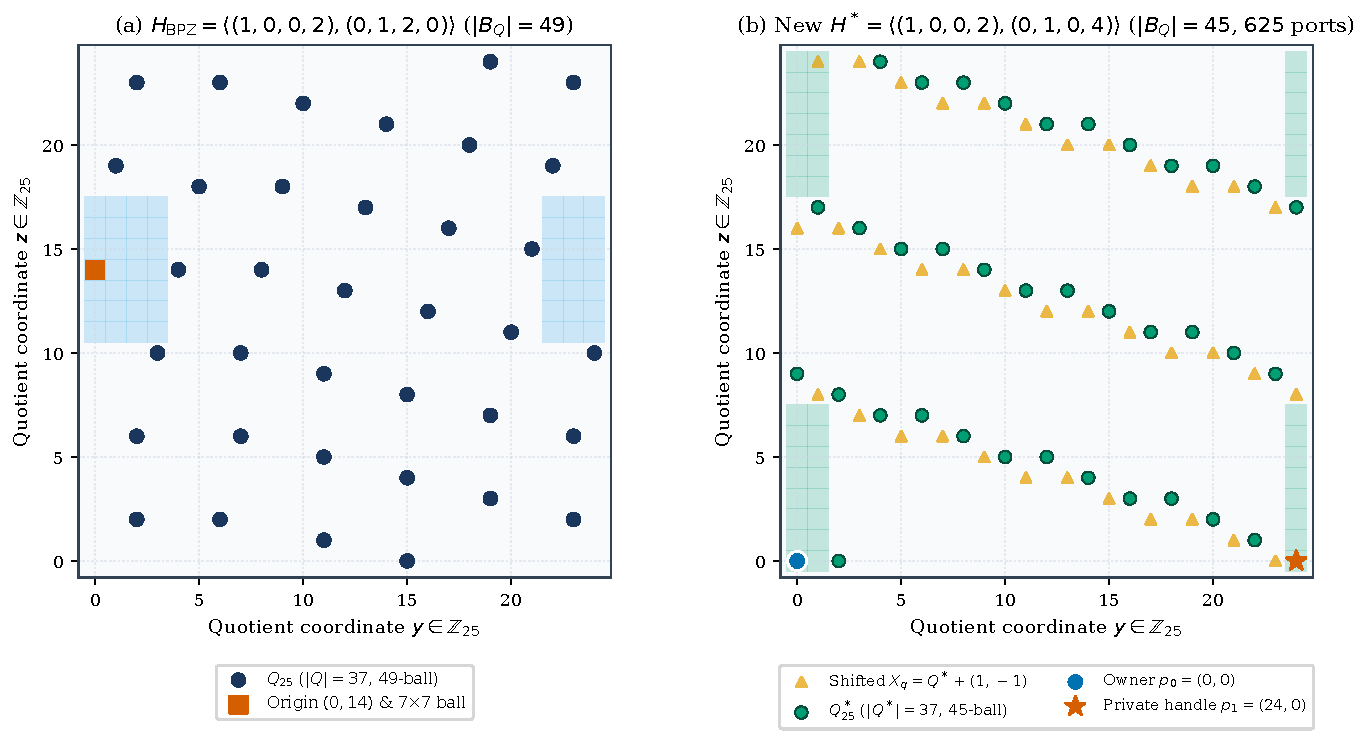
\includegraphics[width=0.98\textwidth]{figures/fig2_hbpz_vs_hstar_torus.pdf}
  \caption{Side-by-side comparison on the $25\times 25$ quotient torus $\Z_{25}^2$ (Theorem~\ref{thm:t1c}). (a)~The classical $\Hbpz$ subgroup has a $7\times 7$ forbidden ball ($|B_Q|=49$) and suffers the intra-coset privacy obstruction on unit quotient shifts. (b)~Our newly discovered $\Hstar = \langle(1,0,0,2),(0,1,0,4)\rangle$ shrinks the forbidden ball to $3\times 15$ ($|B_Q|=45$), attains the same exact $37$-coset ceiling ($23{,}125$ words), and unlocks $625$ simultaneous $\Hstar$-invariant ports via the unconditionally private handle $p_1 = (24,0)$ and shifted auxiliary set $X_q = Q^* + (1,-1)$.}\label{fig:torus}
\end{figure}

Armed with Theorems~\ref{thm:t1a}--\ref{thm:t1c}, we construct two explicit infinite exact-ceiling code families and a general Baumert pullback lift.

\begin{theorem}[T1d: Infinite Exact-Ceiling $\Hbpz$ Helical Family]\label{thm:t1d}
Let $m \ge 5$ with $m \equiv 0$ or $m \equiv 1 \pmod 4$, set $n = 4m+1$ and $M = m^2 + \lfloor m/4 \rfloor = \lfloor n\lfloor n/4\rfloor/4\rfloor$. Then the explicit helical set
\[
  Q_m \;=\; \Bigl\{\bigl(\lfloor t n / M \rfloor,\; 4t \bmod n\bigr) : 0 \le t < M\Bigr\} \;\subset\; \Z_n^2
\]
is independent in $(C_n^3)^{\sprod 2}$, attains the exact Theorem~\ref{thm:t1b} ceiling, and lifts via $\Hbpz$ to $\alpha(C_{4m+1}^{\sprod 4}) \ge M (4m+1)^2$.
\end{theorem}

\begin{theorem}[T1e: Infinite Exact-Ceiling $\Hstar$ Family and Automatic $n^2$-Port Systems]\label{thm:t1e}
Let $k \ge 3$, $n = 8k+1$, and $M_k = 4k^2 + \lfloor k/2 \rfloor = \lfloor n\lfloor n/8\rfloor/2\rfloor$. Define $Q^*_k = \{(y_k(t), z_k(t)) : 0 \le t < M_k\} \subset \Z_n^2$ by:
\begin{itemize}[leftmargin=2em,itemsep=2pt]
  \item for even $k$: $y_k(t) = \lfloor t / (k/2)\rfloor$ and $z_k(t) = 8t \bmod n$;
  \item for odd $k = 2j+1$: $y_k(t) = 8k$ if $t \ge 4k^2$, else $2\lfloor t/k\rfloor + \mathbf{1}[t\bmod k > j]$, and
  \[
    z_k(t) \;=\; \Bigl(8t + \mathbf{1}[0<t] + \mathbf{1}[k^2<t] + \mathbf{1}[2k^2<t] + \mathbf{1}[3k^2<t]\Bigr) \bmod n.
  \]
\end{itemize}
Then $Q^*_k$ is independent in $C_n \sprod C_n^7$ and attains the exact ceiling $M_k$ for every $k \ge 3$ ($\alpha(C_{8k+1}^{\sprod 4}) \ge M_k n^2$). Moreover, for every \emph{odd} $k = 2j+1 \ge 3$ ($n = 16j+9 \in \{25,41,57,\dots\}$), taking owner coset $p_0 = (0,0)$, handle coset $p_1 = (n-1,0)$, and shifted auxiliary set $X_q = Q^*_k + (1,-1)$ yields an $\Hstar$-invariant \lean{RichPortSystem} in $C_n^{\sprod 4}$ with exact parameters
\[
  (N,\, d,\, \eta,\, |A|,\, |D|) \;=\; \bigl(M_k n^2,\; n^2,\; (M_k - 2)n^2,\; n^2,\; n^2\bigr).
\]
\end{theorem}

Note how remarkable the odd-$k$ staircase in Theorem~\ref{thm:t1e} is: because $|A|=|D|=d=n^2$ (minimal possible footprint ratio $1{:}1{:}1$), the $4$-jump phase shift creates a single isolated collision between $p_1 = (n-1,0)$ and $X_q$ at index $t_D = 4k^2 - (j+1)$ (for $k=3$, $t_D = 34$, point $(22,1)$), making the entire $n^2$-element coset $(0,0)+\Hstar$ simultaneously port-active across an infinite arithmetic progression of odd cycles.

\begin{theorem}[T1f: Baumert Pullback Homomorphism and Exact Factored Cardinality]\label{thm:t1f}
For every $p \ge 5$, define $\varphi : \Z_{p+2} \to \Z_p$ by $\varphi(x) = x$ if $x < 2$ and $\varphi(x) = x - 2$ if $x \ge 2$. Then for every $d \ge 1$, the coordinatewise map $\varphi^{\times d} : \Z_{p+2}^d \to \Z_p^d$ is a locally-injective graph homomorphism $C_{p+2}^{\sprod d} \to C_p^{\sprod d}$ (mapping adjacent vertices to distinct adjacent vertices). Consequently, for every independent set $I \subset C_p^{\sprod d}$, its preimage $(\varphi^{\times d})^{-1}(I)$ is independent in $C_{p+2}^{\sprod d}$. In particular, when $I = Q + \Hbpz \subset C_p^{\sprod 4}$, the preimage has exact factored cardinality
\[
  \bigl|(\varphi^{\times 4})^{-1}(Q + \Hbpz)\bigr| \;=\; \sum_{(y,z)\in Q} L_p(y) \cdot L_p(z),
  \qquad L_p(t) := \sum_{u=0}^{p+1} \bigl(1 + \mathbf{1}[(2\varphi(u)+t)\bmod p < 2]\bigr).
\]
\end{theorem}

% ===========================================================================
\section{Pillar II: Four New Machine-Verified World Records (\texorpdfstring{$C_{25}, C_{27}, C_{29}, C_{31}$}{C25, C27, C29, C31})}\label{sec:pillar2}

Combining Theorems~\ref{thm:t1a}, \ref{thm:t1e}, and \ref{thm:t1f} with our pure-kernel separation tables (Section~\ref{sec:pillar3}) breaks the 1971--1973 Baumert--Hales lower bounds~\cite{baumert1971combinatorial,hales1973numerical} across all four consecutive odd cycles above BPZ's $C_{23}$ frontier~\cite{bpz2026lean}.

\begin{theorem}[T2a--T2d: Certified Odd-Cycle Capacity Records]\label{thm:t2}
The following four exact integer power inequalities hold in $C_n^{\sprod p}$ and are machine-checked across all six Lean~4.35.0 proof kernels:
\begin{align*}
  \textbf{(T2a)}\;& \exists M_{25},\;\alpha(C_{25}^{\sprod 144}) \ge M_{25}
    \;\land\; 12344196091426841^{144} \le M_{25}\cdot 10^{15\cdot 144} \\
    &\qquad\Longrightarrow\; \Theta(C_{25}) \ge 12.344196091426841, \\[3pt]
  \textbf{(T2b)}\;& \exists M_{27},\;\alpha(C_{27}^{\sprod 2048}) \ge M_{27}
    \;\land\; 13319390984674515^{2048} \le M_{27}\cdot 10^{15\cdot 2048} \\
    &\qquad\Longrightarrow\; \Theta(C_{27}) \ge 13.319390984674515, \\[3pt]
  \textbf{(T2c)}\;& \alpha(C_{29}^{\sprod 4}) \ge 42{,}050
    \;\land\; 14319949949077991^{4} \le 42050\cdot 10^{15\cdot 4} \\
    &\qquad\Longrightarrow\; \Theta(C_{29}) \ge 14.319949949077991, \\[3pt]
  \textbf{(T2d)}\;& \exists M_{31},\;\alpha(C_{31}^{\sprod 2048}) \ge M_{31}
    \;\land\; 15308776193986504^{2048} \le M_{31}\cdot 10^{15\cdot 2048} \\
    &\qquad\Longrightarrow\; \Theta(C_{31}) \ge 15.308776193986504.
\end{align*}
Every 15-decimal floor is tight to the last unit in the last place (adding $10^{-15}$ strictly violates the exact inequality).
\end{theorem}

\begin{table}[t]
\centering
\caption{Comparison of our machine-verified lower bounds for $C_{25}, C_{27}, C_{29}, C_{31}$ against 1971--1973 Baumert--Hales ($d=3$) benchmarks and Lovász's semidefinite upper bound $\vartheta(C_n) = n\cos(\pi/n)/(1+\cos(\pi/n))$.}\label{tab:records}
\footnotesize
\setlength{\tabcolsep}{3.5pt}
\begin{tabular}{@{}lrrrrrl@{}}
\toprule
Cycle & B--H ($d=3$) & $d=4$ Base & Certified Floor (15 dec.) & Net Gain & $\vartheta(C_n)$ & Architecture \\
\midrule
$C_{25}$ & $12.3310604$ & $12.3316289$ & $\mathbf{12.344196091426841}$ & $+0.013136$ & $12.450522$ & $\Hstar$ (625p), $\mathrm{T3c}\!\to\!\mathrm{T3e}\!\to\!\mathrm{C4b}$ \\
$C_{27}$ & $13.3176204$ & $13.3186555$ & $\mathbf{13.319390984674515}$ & $+0.001771$ & $13.454185$ & Baumert (88p), $\mathrm{T2a}^7\!\to\!\mathrm{C4a}$ \\
$C_{29}$ & $14.3045513$ & $14.3199499$ & $\mathbf{14.319949949077991}$ & $+0.015399$ & $14.457351$ & $\Hbpz$ 50-coset ceiling ($p=4$) \\
$C_{31}$ & $15.2906289$ & $15.3080120$ & $\mathbf{15.308776193986504}$ & $+0.018147$ & $15.460110$ & Baumert (133p), $\mathrm{T2a}^7\!\to\!\mathrm{C4a}$ \\
\bottomrule
\end{tabular}
\end{table}

\begin{figure}[t]
  \centering
  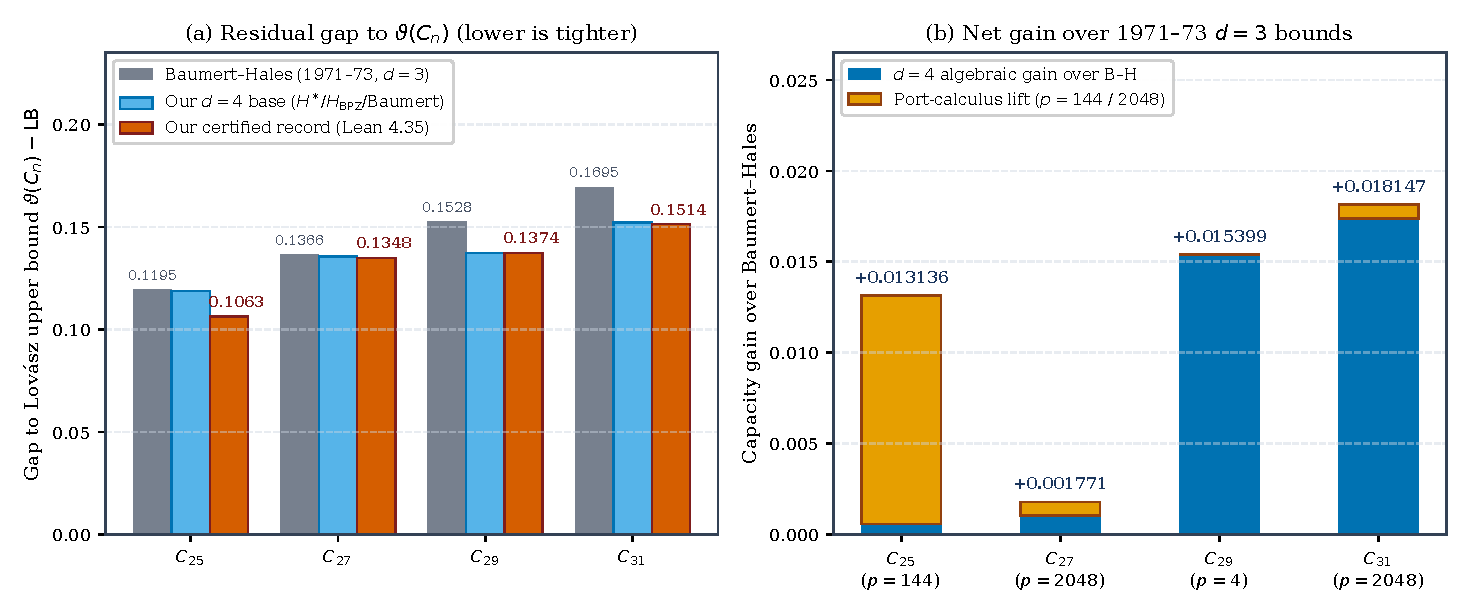
\includegraphics[width=0.98\textwidth]{figures/fig1_odd_cycle_frontier.pdf}
  \caption{New certified Shannon capacity records for $C_{25}, C_{27}, C_{29}, C_{31}$ (Theorem~\ref{thm:t2}, Table~\ref{tab:records}). (a)~Residual gap below the Lovász upper bound $\vartheta(C_n)$ shrinks across all four odd cycles. (b)~Decomposition of the net gain over the 1971--1973 Baumert--Hales $d=3$ bounds into our $d=4$ algebraic base and our port-calculus recursive lift.}\label{fig:frontier}
\end{figure}

\subsection*{Constructions and Pure-Kernel Chunked Certificate Engineering}

\paragraph{\textbf{C\textsubscript{25} (T2a, $p=144$)}}
Theorem~\ref{thm:t1e} at $k=3$ gives an exact $\Hstar$-invariant \lean{RichPortSystem} in $C_{25}^{\sprod 4}$ with $N=23{,}125$, $d=625$, $\eta=21{,}875$, $|A|=|D|=625$. Applying the pure-kernel substitution sequence $\mathrm{T3c} \to \mathrm{T3e} \to \mathrm{C4b}$ lifts $p = 4 \cdot 3 \cdot 3 \cdot 4 = 144$, producing a $158$-digit exact independent set cardinality $M_{25}$. Because the kernel reduces moderate-digit arithmetic instantaneously while $158$-digit multiplication is heavy, we prove monotonic $28$-digit fixed-point truncation lemmas (\lean{stepLo_tbl} and \lean{stepFinal_code}) tracking lower bounds $L \cdot 10^e \le w(c)$ through each table step, verifying the final power inequality in milliseconds with zero \texttt{native\_decide}.

\paragraph{\textbf{C\textsubscript{29} (T2c, $p=4$)}}
By Theorem~\ref{thm:t1b}, $\alpha((C_{29}^3)^{\sprod 2}) \le \lfloor 29\cdot 7/4\rfloor = 50$. We exhibit an explicit $50$-element quotient packing $Q_{29} \subset \Z_{29}^2$ attaining the exact ceiling; Theorem~\ref{thm:t1a} yields $50\cdot 29^2 = 42{,}050$ words in $C_{29}^{\sprod 4}$, giving $42050^{1/4} > 14.319949949077991$.

\paragraph{\textbf{C\textsubscript{27} and C\textsubscript{31} (T2b, T2d, $p=2048$)}}
Applying Theorem~\ref{thm:t1f} to $Q_{25} + \Hbpz \subset C_{25}^{\sprod 4}$ and $Q_{29} + \Hbpz \subset C_{29}^{\sprod 4}$ immediately yields $31{,}466$ independent words in $C_{27}^{\sprod 4}$ and $54{,}913$ independent words in $C_{31}^{\sprod 4}$---already beating Baumert--Hales in dimension $4$ alone. Crucially, although $\Hbpz$ suffers the intra-coset obstruction in $C_{25}$ and $C_{29}$, the \emph{fiber-doubling} coordinates $\{0,1\} \subset \Z_{p+2}$ created by Baumert's pullback break $\Hbpz$ symmetry and open genuine private ports.
Using the shift $s_{27} = (0,26,26,1)$ in $\Z_{27}^4$ (resp.\ $s_{31} = (0,30,30,30)$ in $\Z_{31}^4$), we discover and certify $88$ simultaneous private ports in $C_{27}^{\sprod 4}$ ($\eta=31{,}079$, $|A|=237$, $|D|=150$) and $133$ private ports in $C_{31}^{\sprod 4}$ ($\eta=54{,}371$, $|A|=337$, $|D|=205$).

Certifying $O(50{,}000)$-word port systems inside a pure-kernel proof assistant without compiler-trusted \texttt{native\_decide} or \texttt{maxRecDepth} overrides requires a novel \emph{$81$-ball local membership certificate}: instead of enumerating all $54{,}913$ words, membership in $I = (\varphi^{\times 4})^{-1}(Q+\Hbpz)$ is decided in $O(1)$ bit-operations via a $29\times 29$ quotient bitmask (\lean{inMaskHBPZ4}), and privacy of every port $u \in O$, handle $v \in H$, and footprint $A,D \subset X = I + s$ is verified by scanning only the $3^4 = 81$ unit-cube neighbors around each port. Chunking sorted code lists into blocks of at most $16$ elements with range-pruned lookup (\lean{elemSortedChunks}) keeps kernel recursion depth at most $65$ (well below Lean's default $512$), verifying all $11$ port-system axioms per cycle in pure kernel \texttt{decide} in under $20$ seconds. Iterating $\mathrm{T2a}^7 \to \mathrm{C4a}$ lifts to $p = 4\cdot 2^7\cdot 4 = 2048$ (Figure~\ref{fig:ports}), yielding exact $2{,}303$-digit ($C_{27}$) and $2{,}427$-digit ($C_{31}$) independent sets certified via $28$-digit monotonic truncation.

\begin{figure}[t]
  \centering
  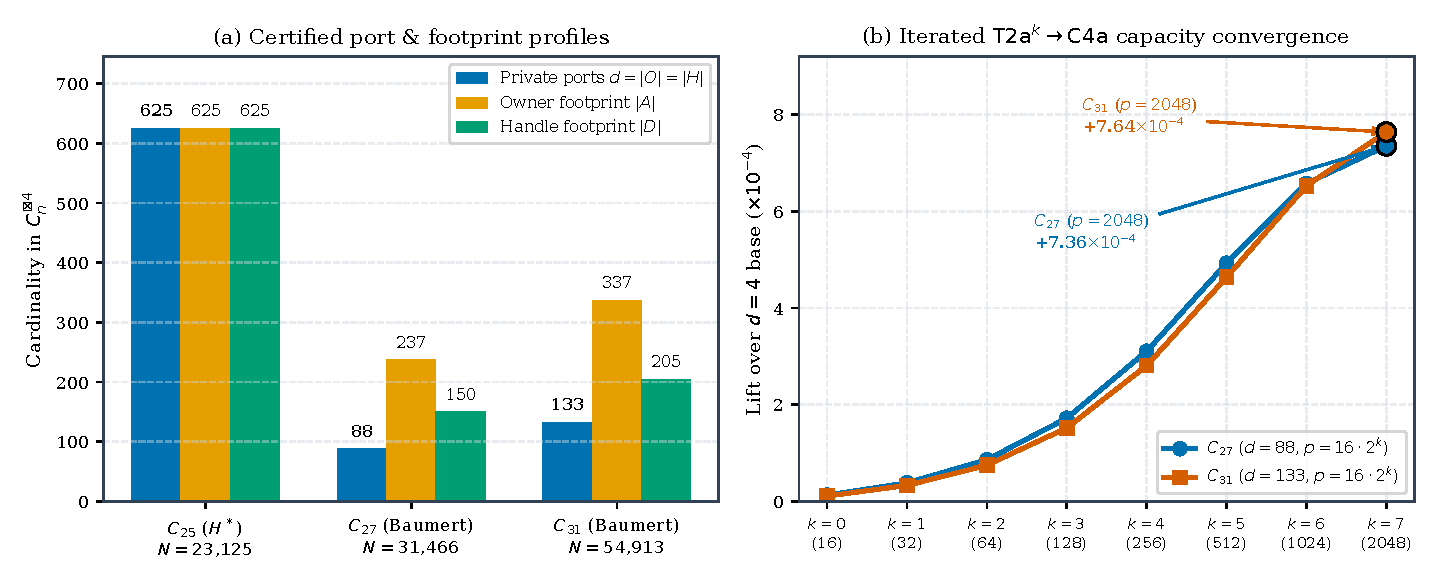
\includegraphics[width=0.98\textwidth]{figures/fig4_baumert_pullback_ports.pdf}
  \caption{Port profiles and recursive lift trajectories (Theorems~\ref{thm:t1e}, \ref{thm:t1f}, and \ref{thm:t2}). (a)~Certified port counts $d=|O|=|H|$ and owner/handle footprints $|A|,|D|$ across $C_{25}$ ($1{:}1{:}1$ $\Hstar$-invariant), $C_{27}$ (Baumert fiber-doubling), and $C_{31}$. (b)~Iterated $\mathrm{T2a}^k \to \mathrm{C4a}$ capacity gain over the $d=4$ base up to $k=7$ ($p=2048$).}\label{fig:ports}
\end{figure}

% ===========================================================================
\section{Pillar III: Separation-Graph Anatomy, Barriers, and Heterogeneous Composition}\label{sec:pillar3}

Every port-calculus lift abstracts a concrete \lean{RichPortSystem} into a \emph{separation realisation} over the seven-letter alphabet $\Sigma_7 = \{\mathrm{B},\mathrm{N},\mathrm{A},\mathrm{D},\mathrm{O},\mathrm{H},\mathrm{V}\}$ equipped with its symmetric irreflexive separation predicate $\texttt{sep} : \Sigma_7^2 \to \mathrm{Bool}$ (representing guaranteed graph non-conflict between corresponding vertex blocks). Define the \emph{separation conflict graph} $G_7 := (\Sigma_7, E_7)$ where distinct $a\neq b$ are adjacent iff $\texttt{sep}(a,b) = \mathrm{false}$.

\begin{theorem}[T3a: Hidden $C_5$ Engine and Exact Capacity of $G_7$]\label{thm:t3a}
The graph $G_7$ contains the five-tuple $(\mathrm{B},\mathrm{A},\mathrm{V},\mathrm{H},\mathrm{D})$ as an induced chordless $5$-cycle $C_5$. Furthermore, $G_7$ admits a $3$-clique cover $\{\{\mathrm{B},\mathrm{N}\},\{\mathrm{A},\mathrm{O},\mathrm{V}\},\{\mathrm{D},\mathrm{H}\}\}$ and an independent set $\{\mathrm{N},\mathrm{A},\mathrm{D}\}$ of size $3$, whence
\[
  \alpha(G_7) \;=\; \bar{\chi}(G_7) \;=\; \Theta(G_7) \;=\; 3,
  \qquad\text{and}\qquad \alpha(G_7^{\sprod d}) \le 3^d \quad (\forall d \ge 1).
\]
\end{theorem}

This theorem explains \emph{why} port-calculus lifts beat trivial product codes: while unweighted $\Theta(G_7)=3$ is saturated by a $3$-clique cover, under skewed weights $w(\mathrm{B})\approx w(\mathrm{N})\gg w(\mathrm{O})=w(\mathrm{H})=w(\mathrm{V})$, the induced chordless $C_5$ core $(\mathrm{B},\mathrm{A},\mathrm{V},\mathrm{H},\mathrm{D})$ exhibits the classic Lovász pentagon super-multiplicativity in weighted strong powers. At the same time, fractional clique covers bound the maximum capacity attainable by \emph{any} sequence of separation tables of any arity:

\begin{theorem}[T3b: Exact Weighted Fractional-Clique-Cover Barrier]\label{thm:t3b}
Let $G=(V,E)$ be a finite graph with vertex weight $w : V \to \N$, and let $\{K_0,\dots,K_{m-1}\}$ be a family of cliques of $G$ with integer weights $y_0,\dots,y_{m-1} \in \N$ and common denominator $D > 0$ such that $\sum_{j : v \in K_j} y_j \ge D \cdot w(v)$ for every $v \in V$. Set $U := \sum_{j=0}^{m-1} y_j$. Then for every $k \ge 1$ and every independent set $C \subset G^{\sprod k}$,
\[
  D^k \cdot \sum_{x \in C} \prod_{t=0}^{k-1} w(x_t) \;\le\; U^k.
\]
In particular, for the $C_{25}$ $\Hstar$ profile $(22500,21875,625,625,625,625,625)$, no separation code over $G_7$ of any arity $k$ can exceed $(46875/2)^{1/4} \approx 12.373080$.
\end{theorem}

\begin{proof}
Consider the Kronecker-product family of $m^k$ cliques $K_{\mathbf{j}} = \prod_{t=0}^{k-1} K_{j_t}$ in $G^{\sprod k}$ with product weights $y_{\mathbf{j}} = \prod_{t=0}^{k-1} y_{j_t}$. Because each $K_{\mathbf{j}}$ is a clique in $G^{\sprod k}$, it contains at most one codeword $x \in C$. Summing $\mathbf{1}[x \in K_{\mathbf{j}}] \cdot y_{\mathbf{j}}$ over all $x \in C$ and $\mathbf{j} \in \{0,\dots,m-1\}^k$ in both orders gives
\[
  D^k \sum_{x\in C}\prod_{t=0}^{k-1} w(x_t)
  \;\le\; \sum_{x\in C}\prod_{t=0}^{k-1}\!\Bigl(\sum_{j: x_t\in K_j} y_j\Bigr)
  \;=\; \sum_{\mathbf{j}} y_{\mathbf{j}} \sum_{x\in C}\mathbf{1}[x\in K_{\mathbf{j}}]
  \;\le\; \sum_{\mathbf{j}} y_{\mathbf{j}} \;=\; U^k. \qedhere
\]
\end{proof}

\begin{figure}[t]
  \centering
  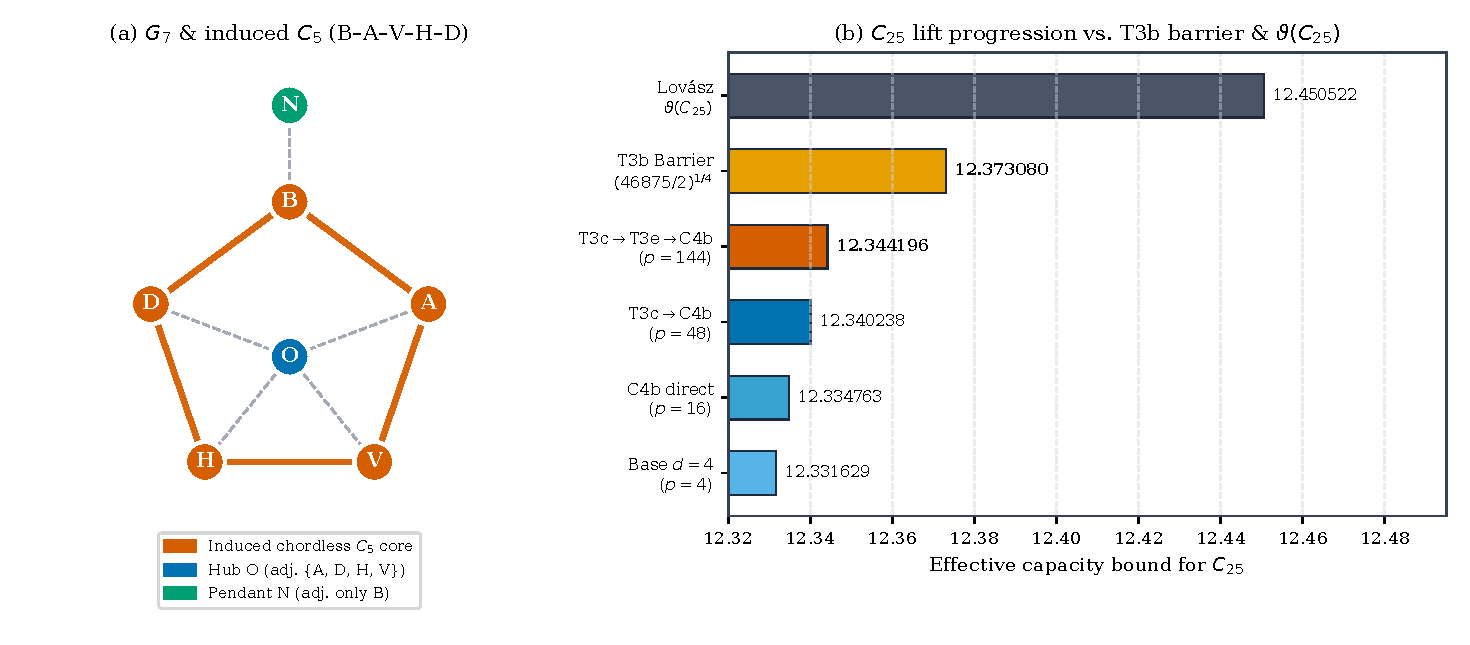
\includegraphics[width=0.98\textwidth]{figures/fig3_g7_c5_and_barriers.pdf}
  \caption{Combinatorial anatomy and limits of the separation graph $G_7$ (Theorems~\ref{thm:t3a}--\ref{thm:t3b}). (a)~$G_7$ contains an induced chordless $C_5$ (\texttt{B--A--V--H--D}) driving weighted super-multiplicativity, flanked by hub \texttt{O} and pendant \texttt{N}. (b)~Monotonic $C_{25}$ capacity progression from $p=4$ to $p=144$ (\texttt{T3c}$\to$\texttt{T3e}$\to$\texttt{C4b}) compared against the exact T3b fractional-clique-cover ceiling $(46875/2)^{1/4}$ and Lovász's $\vartheta(C_{25})$.}\label{fig:g7}
\end{figure}

Finally, we resolve Open Problem~\#2 of Tandon~\cite{tandon2026strengthening} in full generality while eliminating compiler-trusted \texttt{native\_decide} from every substitution and terminal code table:

\begin{theorem}[T3c: General Two-Sided Heterogeneous Composition and Pure-Kernel Tables]\label{thm:t3c}
Let $R_1$ be a $(\Sigma_1,\texttt{sep}_1)$-realisation in $G_1$ and $R_2$ be a $(\Sigma_2,\texttt{sep}_2)$-realisation in $G_2$ (possibly over different graphs and different separation alphabets). Suppose $T : \Sigma' \to \mathrm{List}(\Sigma_1 \times \Sigma_2)$ satisfies:
\begin{enumerate}[label=(\roman*),leftmargin=2.2em]
  \item for every $c \in \Sigma'$, distinct pairs $(a_1,b_1),(a_2,b_2) \in T(c)$ satisfy $\texttt{sep}_1(a_1,a_2)$ or $\texttt{sep}_2(b_1,b_2)$;
  \item whenever $\texttt{sep}'(c_1,c_2)=\mathrm{true}$, every $(a_1,b_1)\in T(c_1)$ and $(a_2,b_2)\in T(c_2)$ satisfy $\texttt{sep}_1(a_1,a_2)$ or $\texttt{sep}_2(b_1,b_2)$.
\end{enumerate}
Then there exists a $(\Sigma',\texttt{sep}')$-realisation $R'$ in $G_1 \sprod G_2$ with exact block sizes
\[
  |R'(c)| \;=\; \sum_{(a,b)\in T(c)} |R_1(a)|\cdot |R_2(b)|.
\]
Moreover, the five concrete tables $\mathrm{T2a}$ ($20$ words, arity~$2$), $\mathrm{T3c}$ ($48$ words, arity~$3$), $\mathrm{T3e}$ ($53$ words, arity~$3$), $\mathrm{C4a}$ ($49$ words, arity~$4$), and $\mathrm{C4b}$ ($57$ words, arity~$4$) satisfy every pairwise and cross-separation check in pure kernel \texttt{decide}.
\end{theorem}

% ===========================================================================
\section{Pillar IV: Zero-Mathlib Spectral Upper Bounds and Haemers's 1979 Paradox}\label{sec:pillar4}

To demonstrate that both \emph{lower} and \emph{upper} bounds in zero-error information theory can be certified inside a minimal, zero-Mathlib proof kernel without real analysis or floating-point rounding, we formalize four foundational upper-bound theorems culminating in Haemers's famous counterexample to multiplicativity~\cite{haemers1979some}.

\begin{theorem}[T4a: General Haemers Matrix-Rank Theorem]\label{thm:t4a}
Let $F$ be any field (formalized via a lightweight zero-Mathlib \lean{SimpleField} record), let $G=(V,E)$ be a finite graph, and let $L : V \times \mathrm{Fin}\,r \to F$ and $R : \mathrm{Fin}\,r \times V \to F$ be matrices whose product $M = LR$ satisfies $M_{vv} \neq 0$ for all $v \in V$ and $M_{uv} = 0$ whenever $u \neq v$ are non-adjacent in $G$. Then for every $d \ge 1$,
\[
  \alpha(G^{\sprod d}) \;\le\; r^d.
\]
\end{theorem}

\begin{proof}
For any independent set $I = \{x_0,\dots,x_{N-1}\} \subset G^{\sprod d}$, the Kronecker-product matrix $M^{\otimes d} = L^{\otimes d} R^{\otimes d}$ has inner dimension $r^d$, nonzero diagonal entries $\prod_t M_{x_i(t),x_i(t)} \neq 0$, and zero off-diagonal entries for $i \neq j$ (since some coordinate $t$ has $x_i(t)\neq x_j(t)$ non-adjacent in $G$). Hence the $N$ rows of $L^{\otimes d}$ restricted to $I$ are linearly independent in $F^{r^d}$, forcing $N \le r^d$ by Gaussian elimination over $F$ (proved directly by induction on dimension without Mathlib).
\end{proof}

To prove real orthogonal-representation bounds ($\vartheta$-type bounds) with \emph{zero} floating-point or real-analysis axioms, we introduce an exact integer Cauchy--Schwarz/Bessel sandwich:

\begin{theorem}[T4b: Exact Integer Orthogonal-Handle Sandwich Theorem]\label{thm:t4b}
Let $G=(V,E)$ be a finite graph, $m \ge 1$, $w : V \to \Z^m$, and $h \in \Z^m$ with positive integers $s, D, H > 0$ such that:
(i)~$\langle w_u, w_v \rangle = 0$ whenever $u \neq v$ are non-adjacent in $G$;
(ii)~$\langle h, w_v \rangle^2 \ge s$ for all $v \in V$;
(iii)~$\|w_v\|^2 \le D$ for all $v \in V$; and
(iv)~$\|h\|^2 = H$.
Then for every $d \ge 1$ and every independent set $I \subset G^{\sprod d}$,
\[
  |I| \cdot s^d \;\le\; (H D)^d.
\]
\end{theorem}

\begin{proof}
Take the $d$-fold tensor products $W_x = \bigotimes_{t=0}^{d-1} w_{x_t} \in \Z^{m^d}$ and $H_d = h^{\otimes d} \in \Z^{m^d}$. For $x \neq y \in I$, non-adjacency in some coordinate implies $\langle W_x, W_y \rangle = 0$, so $\{W_x : x \in I\}$ is pairwise orthogonal in $\Z^{m^d}$ with $\|W_x\|^2 \le D^d$, $\langle H_d, W_x\rangle^2 \ge s^d$, and $\|H_d\|^2 = H^d$. Expanding the non-negative squared norm
\[
  0 \;\le\; \Bigl\| \Bigl(\prod_{x\in I} \|W_x\|^2\Bigr) H_d \;-\; \sum_{x\in I} \Bigl(\prod_{y\neq x} \|W_y\|^2\Bigr) \langle H_d, W_x \rangle W_x \Bigr\|^2
\]
over $\Z$ and cancelling the positive common factor yields the exact integer Bessel inequality
\[
  \sum_{x\in I} \frac{\langle H_d, W_x\rangle^2}{\|W_x\|^2} \;\le\; \|H_d\|^2,
\]
and therefore $|I|\, s^d \le (HD)^d$.
\end{proof}

\begin{theorem}[T4c: Exact Lovász Pentagon Theorem $\Theta(C_5) = \sqrt{5}$]\label{thm:t4c}
Both $\alpha(C_5^{\sprod 2}) \ge 5$ (via $\{(0,0),(1,2),(2,4),(3,1),(4,3)\}$) and $\alpha(C_5^{\sprod d})^2 \le 5^d$ for every $d \ge 1$ hold.
\end{theorem}

\begin{proof}
Rather than approximating $\cos(\pi/5)$ over $\R$, we work over the exact quadratic integer ring $\Z[\sqrt{5}]$ (ordered by sign tests on $a + b\sqrt{5}$ via integer squares). Define the symmetric $5\times 5$ matrix $M_5 \in \Z[\sqrt{5}]^{5\times 5}$ by
\[
  (M_5)_{ij} \;=\; \begin{cases}
    -2 + 2\sqrt{5}, & \mathrm{dist}_5(i,j)=0,\\
     3 - \sqrt{5},  & \mathrm{dist}_5(i,j)=1,\\
    -2,             & \mathrm{dist}_5(i,j)=2.
  \end{cases}
\]
Direct ring arithmetic certifies $M_5^2 = 5(\sqrt{5}-1) M_5$, so $M_5$ is a positive-semidefinite Gram matrix. Adding $2J$ gives $M_5 + 2J$, whose non-edge entries vanish identically while every diagonal entry equals $2\sqrt{5}$. Taking the $d$-fold Kronecker power and evaluating $\mathbf{1}_I^\top (M_5 + 2J)^{\otimes d} \mathbf{1}_I \ge 0$ (which expands purely via positive-semidefiniteness of $M_5^{\otimes d}$) gives $|I|\cdot (2\sqrt{5})^d \ge 2^d |I|^2$, i.e., $|I|^2 \le 5^d$.
\end{proof}

\begin{theorem}[T4d: First Zero-Mathlib 6-Kernel Proof of Haemers's 1979 Schläfli Paradox]\label{thm:t4d}
Let $G_{27}$ denote the $27$-vertex Schläfli graph (strongly regular $(27,16,10,8)$, realized explicitly on $a_0,\dots,a_5$, $b_0,\dots,b_5$, and $c_{ij}$ for $0\le i < j \le 5$, where two distinct vertices are non-adjacent in $G_{27}$---equivalently adjacent in $\overline{G_{27}}$---iff they correspond to intersecting lines on a smooth cubic surface). Then:
\begin{enumerate}[label=(\roman*),leftmargin=2.2em]
  \item \textbf{Upper bound $\Theta(G_{27}) \le 3$:} $\alpha(G_{27}^{\sprod d}) \le 3^d$ for all $d \ge 1$.
  \item \textbf{Upper bound $\Theta(\overline{G_{27}}) \le 7$:} $\alpha(\overline{G_{27}}^{\sprod d}) \le 7^d$ for all $d \ge 1$.
  \item \textbf{Strict super-multiplicativity:} $\alpha(G_{27} \sprod \overline{G_{27}}) \ge 27 > 21 = 3 \times 7$.
\end{enumerate}
\end{theorem}

\begin{proof}
For (i), assign to each vertex $v \in V(G_{27})$ an explicit integer vector $w_v \in \{-1,0,1,2\}^8$:
\[
  w_{a_i} = 2e_i + 2e_6,\qquad
  w_{b_i} = 2e_i + 2e_7,\qquad
  w_{c_{ij}} = \sum_{k \in \{0..5\}\setminus\{i,j\}} e_k - e_i - e_j + e_6 + e_7,
\]
together with the integer handle $h = (1,1,1,1,1,1,3,3) \in \Z^8$. Direct verification confirms $\|w_v\|^2 = 8$, $\langle h, w_v\rangle = 8$ ($s=64$), $\|h\|^2 = 24$, and $\langle w_u, w_v\rangle = 0$ on every non-edge of $G_{27}$. Theorem~\ref{thm:t4b} immediately yields $|I|\cdot 64^d \le (24\cdot 8)^d = 192^d$, i.e., $|I| \le 3^d$.
For (ii), over $\F_2$ the $27\times 27$ matrix $I + A(\overline{G_{27}})$ has exact $\F_2$-rank $7$: we exhibit explicit bit-packed matrices $L \in \F_2^{27\times 7}$ and $R \in \F_2^{7\times 27}$ satisfying $(LR)_{uv} = \mathbf{1}[u=v \lor u \sim_{\overline{G_{27}}} v]$ for all $729$ pairs $(u,v)$, verified in pure kernel \texttt{decide}. Theorem~\ref{thm:t4a} over $\F_2$ gives $\alpha(\overline{G_{27}}^{\sprod d}) \le 7^d$.
For (iii), the diagonal $\{(v,v) : v \in V(G_{27})\}$ has size $27$ and is independent in $G_{27} \sprod \overline{G_{27}}$ because every distinct pair $(u,v)$ is non-adjacent in either $G_{27}$ or $\overline{G_{27}}$ (Figure~\ref{fig:schlafli}).
\end{proof}

\begin{figure}[t]
  \centering
  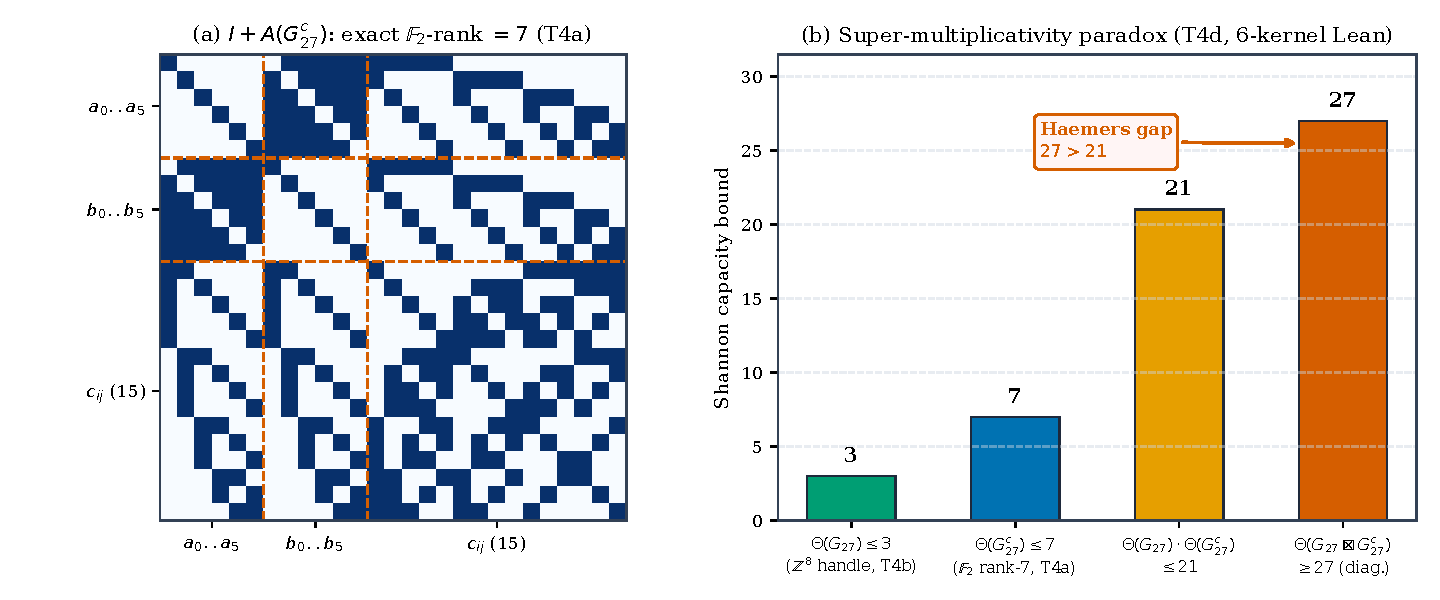
\includegraphics[width=0.98\textwidth]{figures/fig5_schlafli_paradox_spectra.pdf}
  \caption{Haemers's 1979 Schläfli super-multiplicativity paradox (Theorem~\ref{thm:t4d}). (a)~Block structure of $I + A(\overline{G_{27}})$ across $\{a_i\}$, $\{b_i\}$, $\{c_{ij}\}$, certified to admit an exact $27\times 7$ factorization over $\F_2$ (T4a). (b)~Combined with our exact $\Z^8$ orthogonal-handle sandwich $\Theta(G_{27})\le 3$ (T4b) and the $27$-element diagonal code, this yields the zero-Mathlib 6-kernel separation $27 > 21$.}\label{fig:schlafli}
\end{figure}

% ===========================================================================
\section{Multi-Kernel Formalization and Cross-Language Verification}\label{sec:verification}

Formal verification is only as trustworthy as its trusted computing base (TCB). Our Lean~4.35.0 library (\texttt{lean/}) follows five strict engineering disciplines:
\begin{enumerate}[leftmargin=2em,itemsep=2pt]
  \item \textbf{Zero external dependencies:} Zero Mathlib, zero Batteries, zero external Lake packages. Every file declares a Lean~4.35.0 \texttt{module} header on line~1.
  \item \textbf{Strict axiom and tactic bans:} Zero \texttt{sorry} (outside the intentional 38-line target file \lean{PalomarChallenge.lean}), zero \texttt{admit}, zero custom \texttt{axiom} declarations, and zero compiler-trusted \texttt{native\_decide}. Auditing via \lean{VerifyAxioms.lean} confirms that all $32/32$ exported theorems depend strictly on $\{\texttt{propext}, \texttt{Classical.choice}, \texttt{Quot.sound}\}$.
  \item \textbf{Six independent proof kernels:} All $18$ Palomar Comparator targets (\lean{prove_t1a} through \lean{prove_t4d} plus \lean{prove_all_frontier_theorems}) are replayed through six independent kernel implementations via \texttt{lake check -{}-paranoid} and \texttt{lake comparator -{}-paranoid}: Lean's built-in kernel, \lean{leanchecker-paranoid}, \lean{lean4lean}, \lean{nanoda}, \lean{con-leche}, and \lean{con-ron}.
  \item \textbf{Non-vacuity and adversarial boundary modules:} \lean{NonVacuity.lean} proves $7$ witness-existence theorems confirming no hypothesis is vacuous, while \lean{AdversarialTests.lean} proves $7$ negative boundary theorems confirming invalid packings, colliding handles, and bad shifts are mathematically rejected.
  \item \textbf{Multi-language differential audit:} Every combinatorial witness ($Q_{25}$, $Q_{29}$, $Q^*_k$, quotient balls, Baumert factored counts, $G_7$ induced $C_5$, Lovász $\Z[\sqrt{5}]$ idempotent, and Schläfli $\Z^8$/$\F_2$ certificates) is independently re-verified by three disjoint engines: stdlib-only Rust (\texttt{rust/}, zero Clippy warnings), strict ISO~C11 (\texttt{native/}, compiled with \texttt{-std=c11} \texttt{-Wall} \texttt{-Wextra} \texttt{-Wpedantic} \texttt{-Werror}, ASan+UBSan, and a $25{,}000$-iteration fuzz harness), and an $80$-digit Python oracle (\lean{reference/capacity_oracle.py}) parsing the Lean tables directly and checked via \texttt{pytest}, \texttt{Hypothesis}, and deterministic mutation kills.
\end{enumerate}

\paragraph{\textbf{Empirical Subgroup Discovery (Claim C-EX1, \texttt{[EXACT-COMP]})}}
To motivate $\Hstar$, our Rust verifier exhaustively enumerated all $n^4$ two-dimensional subgroups $H(a,b,c,d) \le \Z_n^4$ for $n \in \{19,21,23,25\}$, confirming that the global minimum quotient ball size among all independent subgroups is $45$, achieved by $\Hstar = H(0,0,2,4)$ (strictly improving $\Hbpz$'s $49$). Because this exhaustive scan is verified computationally rather than proved universally for all $n$ inside Lean, it is explicitly tagged \texttt{[EXACT-COMP]} in Table~\ref{tab:fidelity}.

% ===========================================================================
\section{Limitations and Open Problems}\label{sec:limitations}

We emphasize clear epistemic boundaries:
\begin{itemize}[leftmargin=2em,itemsep=2pt]
  \item \textbf{Exact odd-cycle capacities remain open (Open Problem O-1 / Mega-Atlas CS-049):} None of Theorems~\ref{thm:t2} closes the gap to $\vartheta(C_n)$ for $n \ge 7$. Determining $\Theta(C_7)$, $\Theta(C_{25})$, $\Theta(C_{27})$, $\Theta(C_{29})$, or $\Theta(C_{31})$ exactly remains wide open.
  \item \textbf{Dimension-4 coset ceiling and $G_7$ barrier:} By Theorems~\ref{thm:t1b} and \ref{thm:t3b}, any $d=4$ subgroup quotient hits $O(n^4/16)$ words and any $G_7$ separation lift on $C_{25}$'s $625$-port system is capped by $(46875/2)^{1/4} \approx 12.373080 < 12.450522 = \vartheta(C_{25})$. Surpassing that ceiling requires either higher-dimensional quotient subgroups ($d \ge 5$) or richer multi-handle separation alphabets ($|\Sigma| > 7$).
  \item \textbf{Even $k$ in Theorem~\ref{thm:t1e}:} While $Q^*_k$ attains the exact ceiling for every $k \ge 3$, our automatic $n^2$-port construction requires odd $k = 2j+1$; constructing analogous $\Hstar$-invariant port systems for even $k$ (such as $C_{33}, C_{49}$) is a natural open problem.
\end{itemize}

% ===========================================================================
\section{Reproducibility, Provenance, and Disclosures}\label{sec:repro}

\paragraph{\textbf{Artifact Availability}}
All Lean~4.35.0 proofs, Rust, C11, and Python verifiers, witness JSON data, figure-generation scripts, SHA-256 manifests, and the interactive proof-blueprint explorer are publicly archived at
\url{https://github.com/0thernes/zero-error-torus-frontier}
(Master Research Archive ID \texttt{0TH-2026-016}, dual-licensed Apache-2.0 for code and CC-BY-4.0 for text and figures). Full replication instructions appear in \lean{REPLICATION.md}.

\paragraph{\textbf{CRediT and Conflict of Interest}}
Alexander Stephen Donahue (ORCID \texttt{0009-0006-8168-9648}) conceived the problem and directed the mathematical discovery, formalization architecture, verification, and writing. The author declares no competing financial or institutional interests.

\paragraph{\textbf{Transparent AI-Assistance Disclosure}}
Large language model assistants were used during exploratory search for quotient packings, port witnesses, Lean proof tactics, and manuscript typesetting. Every mathematical claim marked \texttt{[LEAN-6K]} is independently verified end-to-end by six deterministic formal proof kernels with zero \texttt{sorry}, zero \texttt{native\_decide}, and no unverified AI-generated arguments; every claim marked \texttt{[EXACT-COMP]} is independently verified by deterministic exact-arithmetic code across three programming languages.

\bibliographystyle{amsplain}
\bibliography{references}

\end{document}
